\subsection{Polar Coordinates}

\ifthenelse{\boolean{teacher}}{
\subsubsection{Introduction}
\begin{itemize}
    \item Up to now we have only studied in a Cartesian coordinate system.
    \begin{itemize}
        \item A Cartesian coordinate system is just a plane described by Cartesian (or, algebraic) equations and points in a finite dimensions.
        \begin{itemize}
            \item \textit{One Dimension}: Lines.
            \item \textit{Two Dimensions}: $x^2$.
            \item \textit{Three, Four}: Upper-level Calculus and Physics.
        \end{itemize}
    \end{itemize}
    \item Let's define an alternative coordinate system --- \textbf{polar coordinate.}
    \begin{itemize}
        \item coordinates are constants on circles and rays.
    \end{itemize}
    \begin{itemize}
        \item Useful for navigation, position, and gravitation fields.
    \end{itemize}
\end{itemize}
}

\subsubsection{Defining Polar Coordinates}
\begin{description}
    \item [Pole] The origin of the coordinate system.
    \item [Polar Axis] Synonymous for the positive $x$-axis.
    \item [Polar Coordinates] A polar coordinates $P$ has the form $(r, \theta)$.
        \begin{description}
            \item [Radial Coordinate] The radial coordinate $r$ describes the \textit{signed}, or \textit{directed}, distance from the origin to $P.$
            \item [Angular Coordinate] The angular coordinate $\theta$ describes an angle whose initial side is the positive $x$-axis and whose terminal side lies on the ray passing through the origin and $P$.
        \end{description}
\end{description}

\ifthenelse{\boolean{teacher}}{
\subsubsection{Notes}
\begin{itemize}
    \item \textbf{Positive angle measurements are measured \textit{counterclockwise} from the origin.}
    \item Every point has multiple representations.
    \begin{itemize}
        \item Angles are periodic, so multiples of $2\pi$ gives the same angle.
        \item Coordinates may be negative. So $(r, \theta)$ can be represented as $(-r, \theta + \pi)$ and $(-r, \theta - \pi)$
    \end{itemize}
\end{itemize}
}

\begin{center}
\begin{tikzpicture}
   \draw[thick,->] (0,0) -- (3,0) node[anchor=north west] {x-axis};
    \draw[thick,->] (0,0) -- (0,3) node[anchor=south east] {y-axis};
    \draw[thick] (0,0) -- (-2,0) node[anchor=north west] {};
    \draw[thick] (0,0) -- (0,-2) node[anchor=south east] {};

    \draw[thick, blue] (0,0) -- (1, 2) node[anchor=north west] {$P(r, \theta), r > 0$};
    \fill[black] (1,2) circle [radius=2pt];

    \draw[thick, thick, red, ->] (.5,0) arc  (.5:15:3cm) ;
    \draw[thick, red] (.65,.5) node{$\theta$};
\end{tikzpicture}
\end{center}

\ifthenelse{\boolean{teacher}}{In summary,}{Some interesting properties to notes.}
\begin{itemize}
    \item $(r, \theta + 2\pi)$ represents the same point as $(r, \theta)$
    \item $P(r, \theta)$ and $P'(-r, \theta)$ are reflections through the origin.
\end{itemize}

\subsubsection{Examples} Graph the following points in polar coordinates:
\begin{itemize}
    \item $Q(1, \frac{5\pi}{3})$
    \item $R(-2, \frac{3\pi}{2})$
    \ifthenelse{\boolean{teacher}}{
    \item $S(3, -\frac{9\pi}{4})$
    \begin{itemize}
        \item Now give two alternative representations.
        \item $S'(3, \frac{1\pi}{4})$
        \item $S''(-3, -\frac{5\pi}{4})$
    \end{itemize}
    }{}
\end{itemize}

\begin{center}
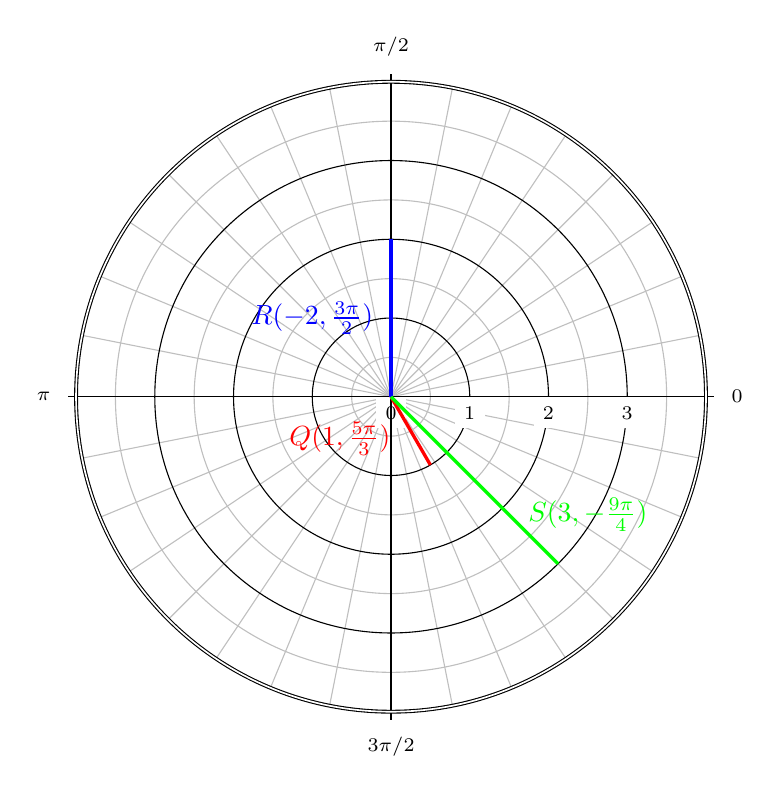
\begin{tikzpicture}[>=latex]
\foreach \ang in {0,...,31} {
  \draw [lightgray] (0,0) -- (\ang * 180 / 16:4);
}

% Concentric circles and radius labels
\foreach \s in {0, 1, 2, 3} {
  \draw [lightgray] (0,0) circle (\s + 0.5);
  \draw (0,0) circle (\s);
  \node [fill=white] at (\s, 0) [below] {\scriptsize $\s$};
}

% Add the labels at multiples of pi/4
\foreach \ang/\lab/\dir in {
  0/0/right,
  2/{\pi/2}/above,
  4/{\pi}/left,
  6/{3\pi/2}/below} {
  \draw (0,0) -- (\ang * 180 / 4:4.1);
  \node [fill=white] at (\ang * 180 / 4:4.2) [\dir] {\scriptsize $\lab$};
}

% The double-lined circle around the whole diagram
\draw [style=double] (0,0) circle (4);

\draw [very thick, red] (0,0) -- (0.5, -0.86602540378444);
\draw [very thick, blue] (0,0) -- (0, 2);


\draw [thick, red] (-0.65, -0.53301270189222) node {$Q(1, \frac{5\pi}{3})$};
\draw [thick, blue] (-1, 1) node {$R(-2, \frac{3\pi}{2})$};

\ifthenelse{\boolean{teacher}}{
\draw [very thick, green] (0,0) --  (2.1213203435596, -2.1213203435596);
\draw [thick, green] (2.5 , -1.5) node {$S(3, -\frac{9\pi}{4})$};}

\end{tikzpicture}
\end{center}

\subsubsection{Converting Between Cartesian and Polar Coordinates}
\ifthenelse{\boolean{teacher}}{
\begin{itemize}
  \item We sometimes need to convert between Cartesian and polar coordinates.
  \item Let's turn this problem into a right triangle.
\end{itemize}

\begin{center}
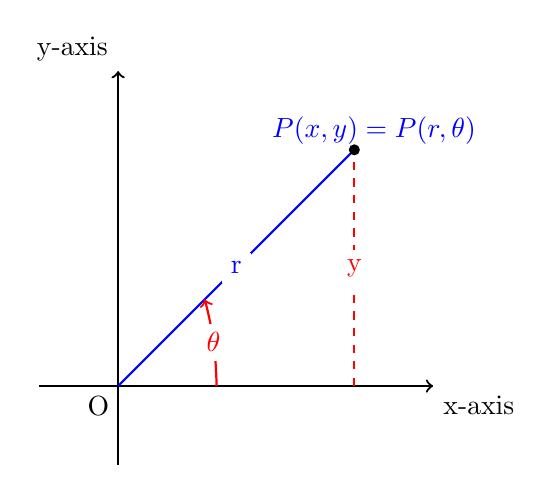
\begin{tikzpicture}
  \draw[thick,->] (0,0) -- (4,0) node[anchor=north west] {x-axis};
  \draw[thick,->] (0,0) -- (0,4) node[anchor=south east] {y-axis};
  \draw[thick] (0,0) -- (-1,0) node[anchor=north west] {};
  \draw[thick] (0,0) -- (0,-1) node[anchor=south east] {};

  \draw[thick] (-.25,-.25) node {O};
  \draw[thick, blue] (0,0) -- (3,3) node[midway, fill=white] {r };

  \draw[thick, dashed, red] (3,0) -- (3,3) node[midway, fill=white] {y};
  \draw[thick, thick, red, ->] (1.25,0) arc  (.5:15:4.4cm) node[midway, fill=white] {$\theta$};

  \fill[black] (3,3) circle [radius=2pt];

  \draw[thick, blue] (3.25,3.25) node {$P(x, y) = P(r, \theta)$};
\end{tikzpicture}
\end{center}
}

A point with polar coordinates $(r, \theta)$ has Cartesian coordinates $(x, y)$, where

\begin{equation}
    x = r \cos \theta \quad \text{and} \quad y = r \sin \theta
\end{equation}

\noindent
A point with Cartesian coordinates $(x, y)$ has polar coordinates $(r, \theta)$, where

\begin{equation}
    r^2 = x^2 + y^2 \quad \text{and} \quad \tan \theta = \frac{y}{x}
\end{equation}


\subsubsection{Examples}
\ifthenelse{\boolean{teacher}}{\textbf{BE SURE TO GRAPH POINTS IN CARTESIAN FIRST.}}{}
\subsubsection{Polar to Cartesian}
Express the point with the following polar coordinates in Cartesian coordinates: $P(3, \frac{2\pi}{3})$
\begin{multicols}{2}
\begin{eqnarray*}
    x & = & r\cos\theta \\
      & = & 3\cos(\nicefrac{2\pi}{3}) \\
      & = & -3(\nicefrac{1}{2}) \\
      & = & -\nicefrac{3}{2}
\end{eqnarray*}

\begin{eqnarray*}
    y & = & r\sin\theta \\
      & = & 3\sin(\nicefrac{2\pi}{3}) \\
      & = & 3(\nicefrac{\sqrt{3}}{2}) \\
      & = & \nicefrac{3\sqrt{3}}{2}
\end{eqnarray*}
\end{multicols}

\ifthenelse{\boolean{teacher}}{
\subsubsection{Polar to Cartesian}
Express the point with the following polar coordinates in Cartesian coordinates: $Q(e, -\frac{\pi}{4})$
\begin{multicols}{2}
\begin{eqnarray*}
    x & = & r\cos\theta \\
      & = & e\cos(-\nicefrac{\pi}{4}) \\
      & = & e(\nicefrac{\sqrt{2}}{2}) \\
      & = & \nicefrac{e\sqrt{2}}{2}
\end{eqnarray*}

\begin{eqnarray*}
    y & = & r\sin\theta \\
      & = & e\sin(-\nicefrac{\pi}{4}) \\
      & = & -e(\nicefrac{\sqrt{2}}{2}) \\
      & = & -\nicefrac{e\sqrt{2}}{2}
\end{eqnarray*}
\end{multicols}
}

\subsubsection{Cartesian To Polar}
Express the point with the following Polar coordinates to Cartesian coordinates: $R(1, -1)$
\begin{multicols}{2}
\begin{eqnarray*}
r & = & \sqrt{x^2 + y^2} \\
  & = & \sqrt{1^2 + (-1)^2} \\
  & = & \sqrt{2}
\end{eqnarray*}

\begin{eqnarray*}
\tan \theta & = & \nicefrac{y}{x} \\
            & = & \nicefrac{-1}{1} \\
            & = & -1 \\
\theta      & = & \nicefrac{-\pi}{4} \ \text{or} \ \nicefrac{7\pi}{4}.
\end{eqnarray*}
\end{multicols}

Therefore, two possible solutions are: $(\sqrt{2}, \nicefrac{-\pi}{4})$ or $(\sqrt{2}, \nicefrac{7\pi}{4})$

\ifthenelse{\boolean{teacher}}{
\subsubsection{Cartesian To Polar}
Express the point with the following Polar coordinates to Cartesian coordinates: $S(1, \sqrt{3})$
\begin{multicols}{2}
\begin{eqnarray*}
r & = & \sqrt{x^2 + y^2} \\
  & = & \sqrt{(\sqrt 3)^2 + (1)^2} \\
  & = & 2
\end{eqnarray*}

\begin{eqnarray*}
\tan \theta & = & \nicefrac{y}{x} \\
            & = & \nicefrac{\sqrt(3)}{1} \\
\theta      & = & \nicefrac{\pi}{3} \ \text{or} \ \nicefrac{4\pi}{3}.
\end{eqnarray*}
\end{multicols}

Therefore, two possible solutions are: $(2, \nicefrac{\pi}{3})$ or $(2, \nicefrac{4\pi}{3})$.
}

\subsubsection{Basic Curves in Polar Coordinates}
\begin{itemize}
    \item A curve in polar coordinates is the set of \textbf{points} that satisfy an equation in $r$ and $\theta$.
    \item This makes graphing some things easier than others.
    \ifthenelse{\boolean{teacher}}{
    \item Look at $r = 3$ is the set of all points that satisfy being away from the origin of $3$ units.
    \begin{itemize}
        \item This is because $\theta$ is not specified, it's arbitrary. Basically, $\theta$ is the function.
        \item In general, $r = a$, $\forall a \in \mathbb{R}^+$ describes a circle.
    \end{itemize}
    \item Taking the converse, let $r$ be arbitrary.
    \begin{itemize}
        \item If the $r$ is arbitrary, and we specify the angle, what do you think we get?
        \item A line!
        \item Take $\nicefrac{\sqrt{2}}{2}$.
    \end{itemize}
    }{}
\end{itemize}

\subsubsection{Polar to Cartesian Graph Example}
Convert the polar equation $r = 6 \sin \theta$ to Cartesian coordinates and describe the corresponding graph.

\begin{eqnarray}
  r^2 & = & 6r\sin\theta \\
  x^2 + y^2 & = & 6y \\
  0 & = & x^2 + y^2 - 6y \\
    & = & x^2 + (y^2 - 6y + 9) - 9  \\
    & = & x^2 + (y- 3)^2 - 9
\end{eqnarray}

We recognize this to be the equation of a circle, centered at $(0, 3)$ at $3$. We can also generalize this.

\subsubsection{Circle in Polar Coordinates}
\begin{itemize}
    \item The equation $r = a$ describes a circle of radius $|a|$ centered at $(0, 0)$.
    \item The equation $r = 2a \sin \theta$ describes a circle of radius  $|a|$ centered at $(0, a)$.
    \item The equation $r = 2a \cos \theta$ describes a circle of radius $|a|$ centered at $(a, 0)$.
\end{itemize}

\begin{multicols}{3}
\centering
\resizebox{.8\columnwidth}{!}{
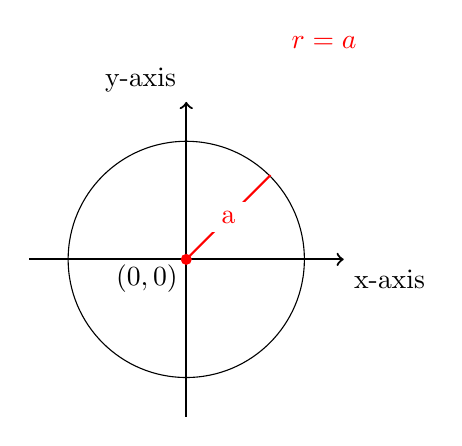
\begin{tikzpicture}
   \draw[thick,->] (0,0) -- (2,0) node[anchor=north west] {x-axis};
    \draw[thick,->] (0,0) -- (0,2) node[anchor=south east] {y-axis};
    \draw[thick] (0,0) -- (-2,0) node[anchor=north west] {};
    \draw[thick] (0,0) -- (0,-2) node[anchor=south east] {};

    \draw (0,0)  circle (1.5cm);
    \draw [thick] (-.50,-.25) node {$(0, 0)$};

    \draw[thick, red] (0,0) -- ++(1.07, 1.07) node[midway, fill=white] {a};
    \fill[red] (0,0) circle [radius=2pt];

    \draw[thick, red] (1.75,2.75) node {$r = a$};
\end{tikzpicture}
}

\resizebox{.8\columnwidth}{!}{
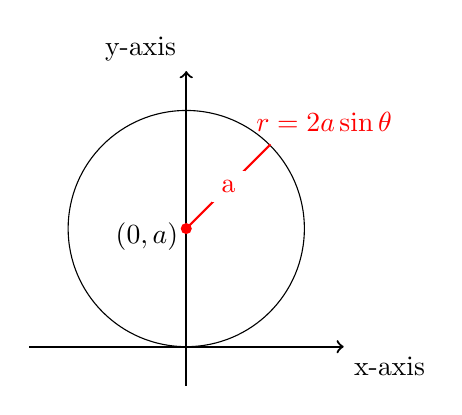
\begin{tikzpicture}
   \draw[thick,->] (0,0) -- (2,0) node[anchor=north west] {x-axis};
    \draw[thick,->] (0,0) -- (0,3.5) node[anchor=south east] {y-axis};
    \draw[thick] (0,0) -- (-2,0) node[anchor=north west] {};
    \draw[thick] (0,0) -- (0,-.5) node[anchor=south east] {};

    \draw (0,1.5)  circle (1.5cm);
    \draw [thick] (-.50,1.40) node {$(0, a)$};

    \draw[thick, red] (0,1.5) -- ++(1.07, 1.07) node[midway, fill=white] {a};
    \fill[red] (0,1.5) circle [radius=2pt];

    \draw[thick, red] (1.75,2.85) node {$r = 2a \sin \theta $};
\end{tikzpicture}
}

\resizebox{.8\columnwidth}{!}{
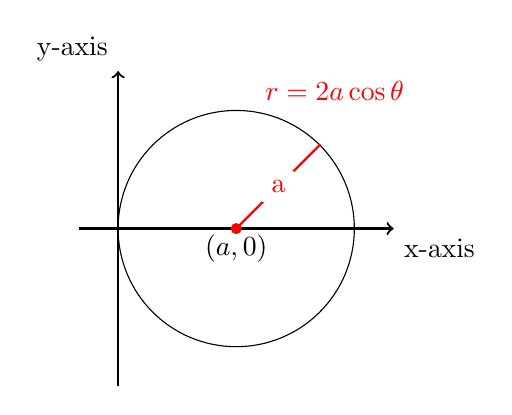
\begin{tikzpicture}
   \draw[thick,->] (0,0) -- (3.5,0) node[anchor=north west] {x-axis};
    \draw[thick,->] (0,0) -- (0,2) node[anchor=south east] {y-axis};
    \draw[thick] (0,0) -- (-.5,0) node[anchor=north west] {};
    \draw[thick] (0,0) -- (0,-2) node[anchor=south east] {};

    \draw (1.5,0)  circle (1.5cm);
    \draw [thick] (1.5,-.25) node {$(a, 0)$};

    \draw[thick, red] (1.5,0) -- ++(1.07, 1.07) node[midway, fill=white] {a};
    \fill[red] (1.5,0) circle [radius=2pt];

    \draw[thick, red] (2.75,1.75) node {$r = 2 a \cos \theta $};
\end{tikzpicture}
}
\end{multicols}

\subsubsection{Graphing In Polar Coordinates}
\ifthenelse{\boolean{teacher}}{
Graph the polar equation $r = f(\theta) = 1 + \sin \theta$

\begin{multicols}{2}
\resizebox{.5\columnwidth}{!}{
\begin{tabular}{c|c}
  \toprule
  \textbf{$\theta$} & \textbf{$r = 1 + sin \theta$} \\ \hline
  0 & 1 \\
  $\nicefrac{\pi}{6}$ & $\nicefrac{3}{2}$ \\
  $\nicefrac{\pi}{2}$ & $2$ \\
  $\nicefrac{5\pi}{6}$ & $\nicefrac{3}{2}$ \\
  $\pi$ & $1$ \\
  $\nicefrac{7\pi}{6}$ & $\nicefrac{1}{2}$\\
  $\nicefrac{3\pi}{2}$ & $0$\\
  $\nicefrac{11\pi}{6}$ & $\nicefrac{1}{2}$\\
  $2\pi$ & $1$\\
\end{tabular}
}

\resizebox{.8\columnwidth}{!}{
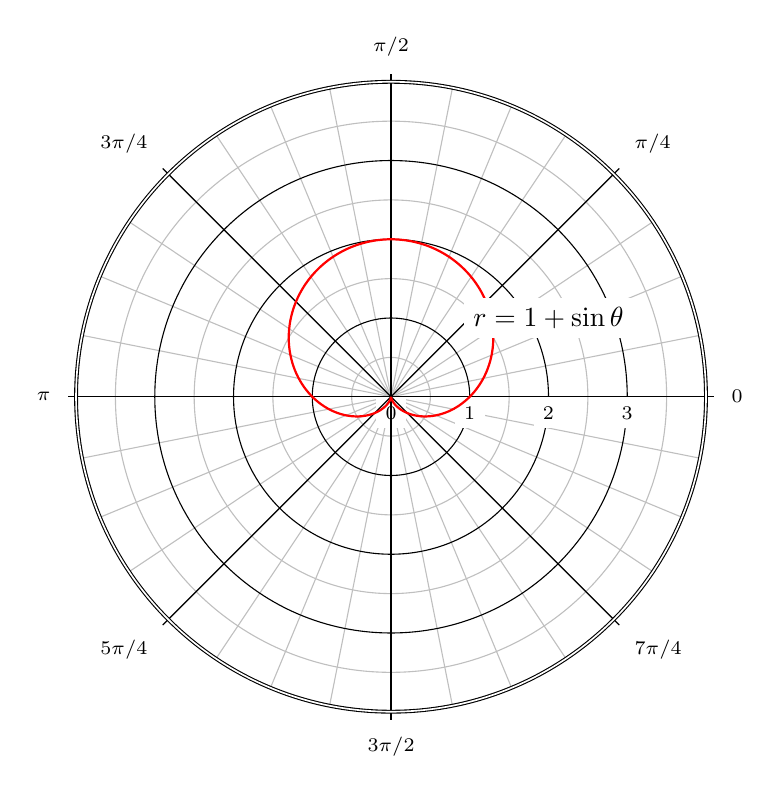
\begin{tikzpicture}[>=latex]
% Draw the lines at multiples of pi/12
\foreach \ang in {0,...,31} {
  \draw [lightgray] (0,0) -- (\ang * 180 / 16:4);
}

% Concentric circles and radius labels
\foreach \s in {0, 1, 2, 3} {
  \draw [lightgray] (0,0) circle (\s + 0.5);
  \draw (0,0) circle (\s);
  \node [fill=white] at (\s, 0) [below] {\scriptsize $\s$};
}

% Add the labels at multiples of pi/4
\foreach \ang/\lab/\dir in {
  0/0/right,
  1/{\pi/4}/{above right},
  2/{\pi/2}/above,
  3/{3\pi/4}/{above left},
  4/{\pi}/left,
  5/{5\pi/4}/{below left},
  7/{7\pi/4}/{below right},
  6/{3\pi/2}/below} {
  \draw (0,0) -- (\ang * 180 / 4:4.1);
  \node [fill=white] at (\ang * 180 / 4:4.2) [\dir] {\scriptsize $\lab$};
}

% The double-lined circle around the whole diagram
\draw [style=double] (0,0) circle (4);

\draw [thick,color=red,domain=0:2*pi,samples=200,smooth] plot (xy polar cs:angle=\x r,radius= {1 + sin(\x r)});
\node [fill=white] at (2,1) {$r=1+\sin\theta$};

\end{tikzpicture}
}
\end{multicols}

The resulting curve is known as a \textbf{cardioid}.
}

\subsubsection{Cartesian-to-Polar Method for Graphing $r = f(\theta)$}
\begin{enumerate}
    \item Graph $r = f(\theta)$ \textit{as if $r$ and $\theta$ were Cartesian coordinates} with $\theta$ on the horizontal axis and $r$ on the vertical axis. Be sure to choose an interval in $\theta$ on which the entire polar curve is produced.
    \item Use the Cartesian graph in Step 1 as a guide to sketch the points $(r, \theta)$ on the final \textit{polar} curve.
\end{enumerate}

\ifthenelse{\boolean{teacher}}{
\subsubsection{Example}
With the alternate graphing method, graph $r = 1 + \sin\theta$.

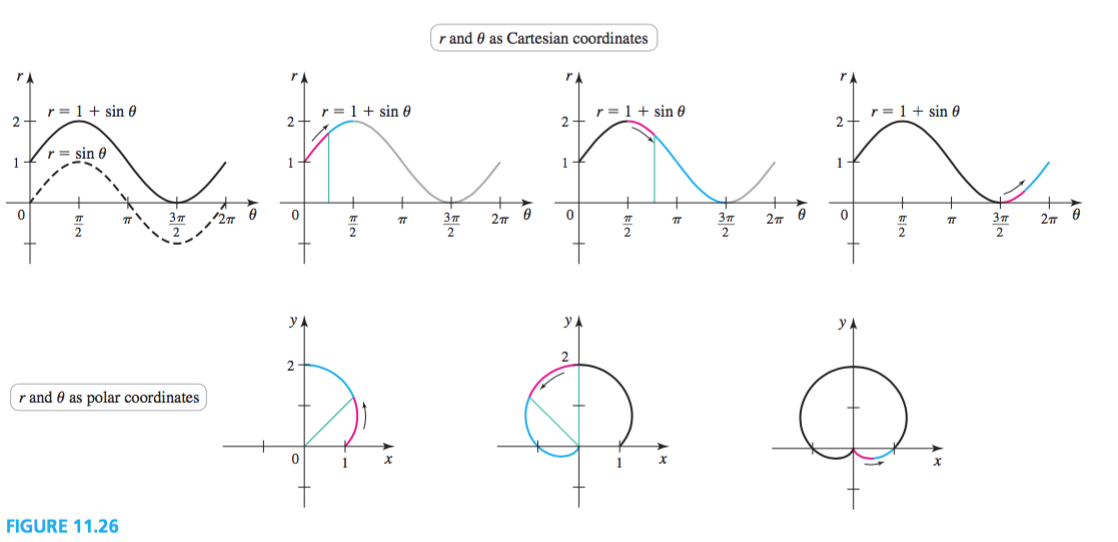
\includegraphics[width=\textwidth]{example}
}

\subsubsection{Symmetry In Polar Equations}
\begin{description}
    \item [Symmetry about the x-axis] occurs if the point $(r, \theta)$ is on the graph whenever $(r, -\theta)$ is on the graph.
    \item [Symmetry about the y-axis] occurs if the point $(r, \theta)$ is on the graph whenever $(r, \pi - \theta) = (-r, -\theta)$ is on the graph.
    \item [Symmetry about the origin] occurs if the point $(r, \theta$ is on the graph whenever $(-r, \theta) = (r, \theta + \pi)$ is on the graph.
\end{description}
